\chapter{XEB的实验实现}
由于具体相关实验我并没有做过,只能复述Google的方案.主要分成两部分,一部分是fSim门的校准,另一个是Google量子称霸线路的简要介绍
\section{fSim门的校准}
整个流程依照的是"Demonstrating a Continuous Set of Two-qubit Gates for Near-term Quantum Algorithms"这篇文章,虽然比特结构有所不同,但是并不影响标定比特的方法.而单比特门就用简单的RB就可以,这里不再赘述
\subsection{测量coupler不同bias下,耦合强度的大小}
在不同coupler的bias下,将两个比特的频率差Δ调为0,观察q-q swap,进行傅里叶变换,得到不同bias下的耦合强度g.实验线路,q-q swap图,以及bias与耦合g的关系图,分别由下图\ref{bias-g}中的a,b,c表示
\begin{figure}
	\centering
	\includegraphics[width=0.8\textwidth]{bias-g}
	\caption{coupler的bias与耦合强度g的关系图} 
	\label{bias-g}
\end{figure}

\textcolor{red}{问题在于:如何确保Δ=0,实验中的crosstalk会导致Δ的改变}
\subsection{fSim门的参数确定}
在进行实验之前,首先要确定我们能控制的参数,对于实际实验来说,因为所有波形都是同步的,而且形状皆为名义上的方波(各种滤波和频率响应的影响),所以主要有四个参数:
\begin{itemize}
	\item 三个波形共同的时间
	\item 比特一波形幅度
	\item 比特二波形幅度
	\item coupler波形幅度
\end{itemize}

而对于这个波形所驱动的演化,对应的演化矩阵有leakage和$\theta,\phi,\Delta_{+},\Delta_{-},\Delta_{-,off}$这五个理想矩阵中的参数
\begin{equation}
\centering 
G=\left[
\begin{array}{cccc}  
1 & 0 & 0 & 0\\ 
0 & e^{(\Delta_{+}+\Delta_{-})}cos(\theta) & -ie^{(\Delta_{+}-\Delta_{-,off})}sin(\theta) & 0\\ 
0 & -ie^{(\Delta_{+}+\Delta_{-,off})}sin(\theta) & e^{(\Delta_{+}-\Delta_{-})}cos(\theta) & 0\\ 
0 & 0 & 0 & e^{i(2\Delta_{+}+\phi)}\\ 
\end{array}
\right ]
\end{equation}
其中$\Delta_{+},\Delta_{-},\Delta_{-,off}$可以通过相位补偿补偿掉,所以主要关注的还是$leakage,\theta,\phi$这三个参数,而这三个参数的测量可以通过下图\ref{leakage_theta_phi}中的a,b,c分别得到
\begin{figure}
	\centering
	\includegraphics[width=0.9\textwidth]{leakage_theta_phi}
	\caption{$leakage,\theta,\phi$的实验测量} 
	\label{leakage_theta_phi}
\end{figure}
然后我们就可以选择合适的detuning和g来获得我们想要的$leakage,\theta,\phi$.这里需要说明的是,一般来说不会直接做整个($\theta,\phi$)空间的fSim,而是将fSim拆成两部分”CPHASE”,” iSWAP-like”
\begin{itemize}
	\item CPHASE:$\phi$可以从0取到360,也会积累比较小的$\theta$($\theta \leq 5$)
	\item iSWAP-like:$\theta$能从0积累到90,但还是会有$\phi$积累($\phi \propto \theta^{2}$)
\end{itemize}
通过这两部分,我们达到整个($\theta,\phi$)空间

我们还提出一种方法可以直接测量$\theta,\phi,\Delta_{+},\Delta_{-},\Delta_{-,off}$这五个参数的方法.对于一个photon conserving的演化中,演化矩阵可以写成下面这种形式:
\begin{equation}
\centering 
G=\left[
\begin{array}{cccc}  
1 & 0 & 0 & 0\\ 
0 & u_{11} & u_{12} & 0\\ 
0 & u_{21} & u_{22} & 0\\ 
0 & 0 & 0  & u_{33}\\ 
\end{array}
\right ]
\end{equation}


我们可以用下面表格\ref{para_mearuse}所示的方法,来确定$u_{11},u_{12},u_{21},u_{22},u_{33}$
\begin{figure}
	\centering
	\includegraphics[width=0.9\textwidth]{para_mearuse}
	\caption{$\theta,\phi,\Delta_{+},\Delta_{-},\Delta_{-,off}$参数测量方法} 
	\label{para_mearuse}
\end{figure}
其中initial state代表如何制备初态,X代表将对应比特激发,0为基态,1为激发态,然后施加fSim,在measure qubit中,0,1分别代表对第一个和第二个比特进行测量,测量$σ_{X}+iσ_{Y}$,就可以得到对应的u的复数.然后通过对应的u和五个参数之间的关系,如下表\ref{para_u}所示,就可以得到演化矩阵中对应的参数$\theta,\phi,\Delta_{+},\Delta_{-},\Delta_{-,off}$
\begin{figure}
	\centering
	\includegraphics[width=0.9\textwidth]{para_u}
	\caption{u和各矩阵参数对应关系} 
	\label{para_u}
\end{figure}

这种方法由于制备和测量的精度,只能到$10^{-3}$的精度
\subsection{fSim门的实验校准}
通过上面fSim门的参数确定,我们可以得到保真度比较高的单个CPHASE或者iSWAP-like.但是由于拖尾的原因,我们很难得到保真度高的组合起来的fSim门,而且前一个双比特门也会影响下一个双比特门,这时我们就需要对拖尾进行校准.

这里我们主要校准的是较长时间的拖尾,也就是两个fSim门之间的互相影响.至于fSim门内部两个门之间的拖尾的影响则不再拖尾校准考虑范围里,主要是通过两种方法进行消除:
\begin{itemize}
	\item 当连续施加两个门时,施加的第二个门的幅度要根据第一个门进行改变,也就是在参数确定时,确定第二个门的参数要考虑第一个门
	\item 当又施加CPHASE又施加iswap-like时,先CPHASE后iswap-like,否则泄露会比较大
\end{itemize}
而拖尾对门本身波形导致的形变,因为整个效应的大小主要由积分来确定,所以波形的略微形变对结果影响很小.因此难点是对影响两个fSim门之间的拖尾进行校准.

首先介绍如何校准单个\textbf{CPHASE门}:
\begin{itemize}
	\item[1] 制备11态,当比特频率间距∆在非简谐η附近,对于每一个∆,不断改变coupler的pulse的强度,直到测得的leakage最小,得到$amp_{c}$
	\item[2] 对于每一组∆,$amp_{c}$,测量对应的$\theta,\phi,\Delta_{+},\Delta_{-},\Delta_{-,off}$,就可以测到一组合适的CPHASE门
\end{itemize}

然后介绍如何校准单个$\theta=90$的\textbf{iswap-like门}:
\begin{itemize}
	\item[1] 制备10态,先设定比特方波强度$amp_{q1}$和$amp_{q2}$使得名义上共振,然后调节coupler方波强度$amp_c$使得振幅最大,如下图\ref{iswap}(a)所示
	\item[2] 制备10态,通过确定的$amp_c$,改变$amp_{q1}$和$amp_{q2}$使得振幅最大,使其共振,确定$amp_{q1}$和$amp_{q2}$,如下图\ref{iswap}(b)所示
	\item[3] 已经确定了$amp_{q1}$和$amp_{q2}$,通过改变$amp_c$,使得振幅最大,确定最终的$amp_c$,如下图\ref{iswap}(c)所示
\end{itemize}
\begin{figure}
	\centering
	\includegraphics[width=0.4\textwidth]{iswap}
	\caption{$\theta=90$的iswap-like门校准} 
	\label{iswap}
\end{figure}

最后介绍如何校准合成的\textbf{fSim门}:
\begin{itemize}
\item[1] 利用标定CPHASE门的方法,按条件相位,从0到360每一度标定一个CPHASE门,如下图\ref{fsim}(a)所示
\item[2] 在(1)中标定的每一种CPHASE门后加iswap-like门,分别标定实现θ=0或90的两种iswap-like门,如下图\ref{fsim}(b)所示
\item[3] 对于φ=180的CPHASE,标定后面的θ从0到90的每一度一个iswap-like门,如下图\ref{fsim}(b)所示
\end{itemize}
其余的部分就是插值得到.
\begin{figure}
	\centering
	\includegraphics[width=0.8\textwidth]{fsim}
	\caption{fsim门校准} 
	\label{fsim}
\end{figure}


对于两个fSim门之间的校准,主要依靠电子学上的校准.对于比特,校准方式与我们相似,制备正态,测量拖尾积累的相位得到响应函数,然后利用三个指数decay time进行拟合.对于coupler,现在并没有原位的校准技术,只能将相邻比特的拖尾模型参数的平均值作为coupler的拖尾模型参数.


\section{Google量子称霸实现的简要介绍}
谷歌量子称霸方法的逻辑依据只有两条:
\begin{itemize}
	\item[1] 量子线路保真度主要受到量子门的数量和质量的影响	
	\item[2] 经典仿真的复杂度对于门线路的结构很敏感
\end{itemize}

首先需要说明的是,如下图\ref{architecture}所示,中间红色部分的coupler将左右两部分相连接,所以这部分coupler所做的iSwap-like门越多,两侧的联系越紧密,无论是用Schrödinger algorithm还是Schrödinger–Feynman进行经典计算,复杂度都会大大增加.如果减少这部分的CZ门,会让经典计算复杂度大大降低,但是对整个量子线路的保真度其实影响很小.
\begin{figure}
	\centering
	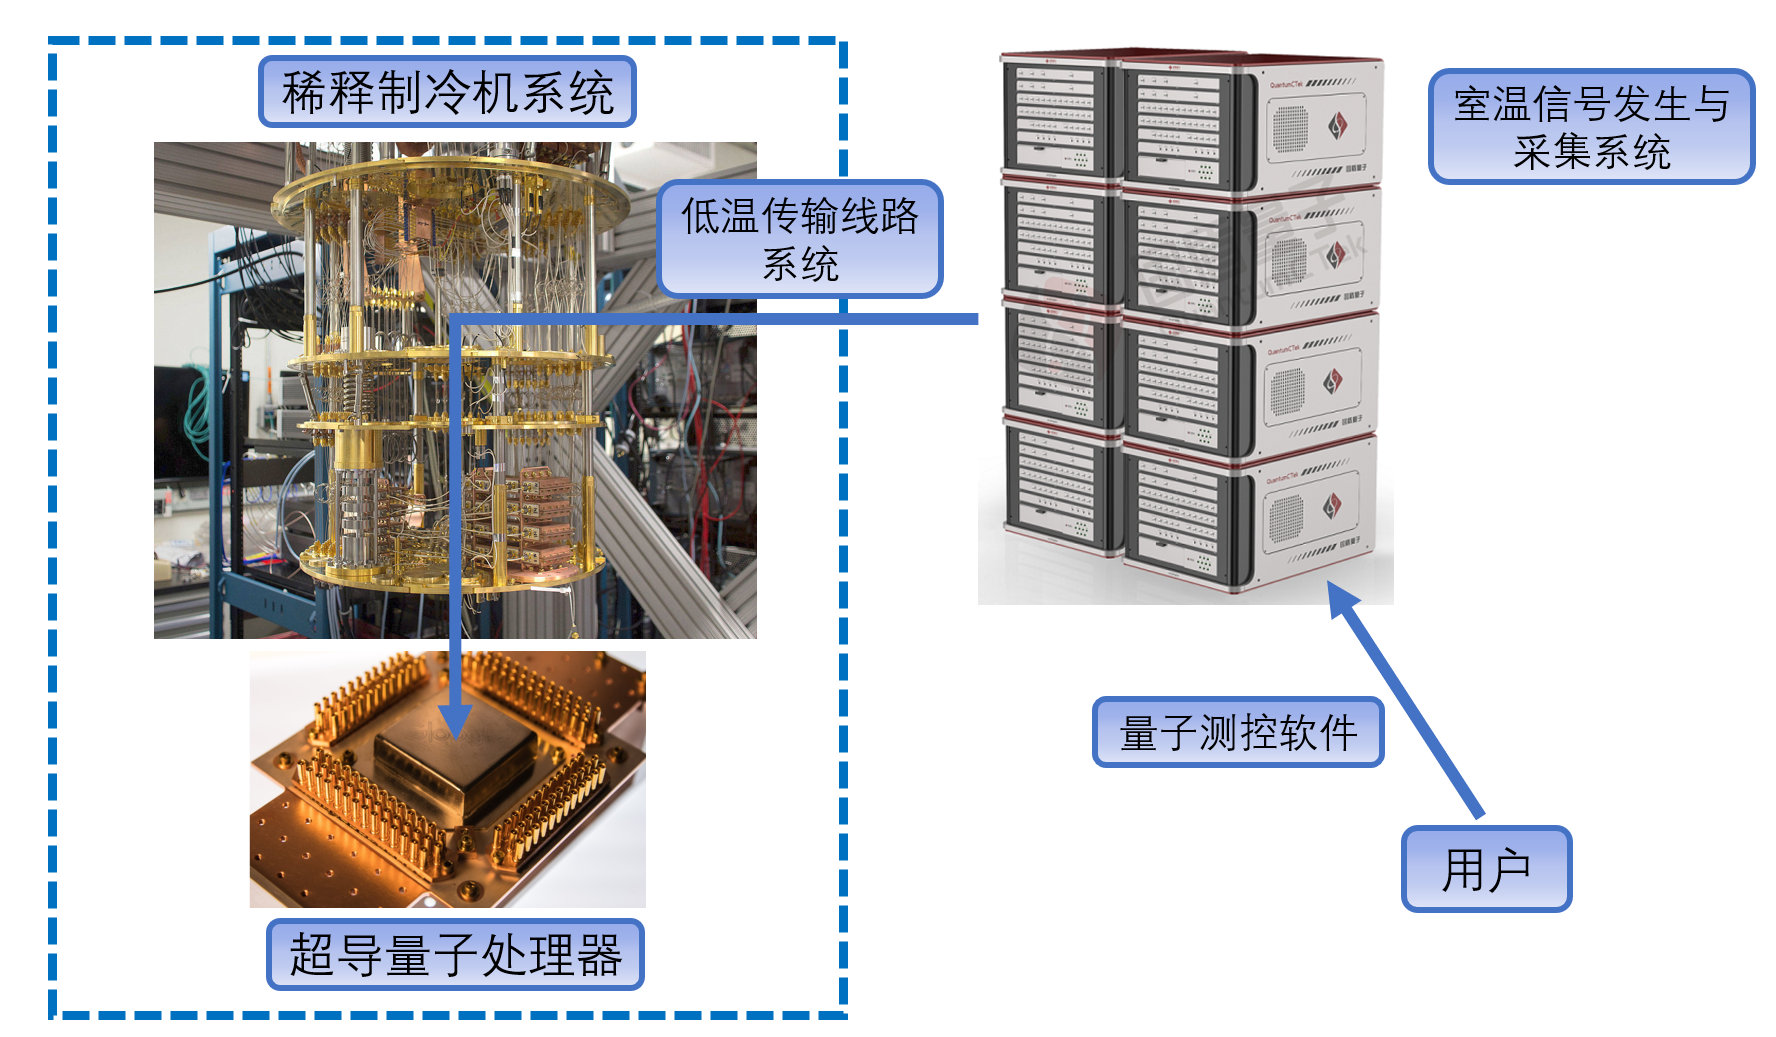
\includegraphics[width=0.7\textwidth]{architecture}
	\caption{53比特结构} 
	\label{architecture}
\end{figure}

以此为依据,Google设计了elided circuits和patch circuits,门的数目如下表\ref{gate_count}所示
\begin{figure}
	\centering
	\includegraphics[width=0.8\textwidth]{gate_count}
	\caption{不同线路们的数目} 
	\label{gate_count}
\end{figure}

其中可以看出,对于patch circuits,交接红色部分(Cross-partition)的双比特门全部取消,所以经典计算复杂度大大降低,但是门的数目改变比例相对较小,所以利用XEB估计的保真度与完整的full circuits相差比较小;对于elided circuits,交接红色部分(Cross-partition)的双比特门仅仅有所减少,所以经典计算复杂度大大降低,但是门的数目改变比例很低,所以利用XEB估计的保真度与完整的full circuits相差应该更小,是用来估计full circuits的良好线路(其中简化的三种线路是改变了参数比特数目和线路深度,用以进行保真度的验证).因此设计了如图\ref{experiment}实验:
\begin{figure}
	\centering
	\includegraphics[width=0.7\textwidth]{experiment}
	\caption{量子称霸实验} 
	\label{experiment}
\end{figure}

首先在更少的比特上,分别使用十四层深度的简化patch circuits,简化elided circuits,简化full circuits,利用XEB得到的保真度如图\ref{experiment}(a)中所示,几个保真度都是在误差范围内是重合的,所以我们可以利用elided circuits来对full circuits的保真度进行估计.以此为依据完成了完整的53个比特,20个cycles的elided circuits,这种简化了的线路是可以用经典计算机计算理论的$p_{s}(q)$,因此可以利用XEB计算整个线路的保真度,并以这个elided circuits的保真度作为无法使用XEB计算保真度的full circuits的保真度.这样我们就得到一个保真度显著大于0的量子线路,使用经典计算机模拟需要10000年,完成了量子称霸
